\documentclass[aspectratio=169]{beamer}
\usepackage{caption}

\captionsetup[algorithm]{labelformat=empty}
\setbeamertemplate{title page}[default][left] % left-align title page (commend out for centered title page)
\beamertemplatenavigationsymbolsempty % remove navigation symbols

\usepackage{fontspec}
\usepackage{sourcesanspro}
\usepackage[T1]{fontenc}

% TODO: albatian
\usefonttheme{serif}
\usefonttheme{professionalfonts}
\usepackage{mathtools}
\usepackage[tracking=true]{microtype}

\usepackage{bold-extra}
\usepackage{realscripts}
\usepackage{amsmath,bm,amssymb}
\usepackage{amsthm}
\usepackage{bbm}
\usepackage{tikz}
\usepackage[group-digits=integer,group-minimum-digits=4,group-separator={,},detect-all]{siunitx}
\usepackage{algorithmicx}
\usepackage{algorithm}
\usepackage{textpos}
\usepackage{xcolor}
\usepackage{multirow}
\usepackage{longtable,tabularx,booktabs}
\usepackage[flushleft]{threeparttable}
\usepackage{vector} % local
\usepackage{varwidth}


%%%%%%%%%%%%%%%%%%%%%%%%%%%%%%%%%%%%%%%%%%%%%%%%%%
% Unicode settings
%%%%%%%%%%%%%%%%%%%%%%%%%%%%%%%%%%%%%%%%%%%%%%%%%%
\setmonofont{DejaVu Sans Mono}[Scale=MatchLowercase]
\usepackage{newunicodechar}
\newfontface{\calligraphic}{Latin Modern Math}[Scale=0.85]
\newunicodechar{𝒪}{{\normalfont\calligraphic 𝒪}}
\newunicodechar{ℬ}{{\normalfont\calligraphic ℬ}}
\newunicodechar{𝒜}{{\normalfont\calligraphic 𝒜}}
\newunicodechar{𝒟}{{\normalfont\calligraphic 𝒟}}
\newunicodechar{𝒮}{{\normalfont\calligraphic 𝒮}}
\newunicodechar{𝔼}{{\normalfont\calligraphic 𝔼}}
\newunicodechar{⋮}{{\normalfont ⋮}}
\newunicodechar{φ}{ϕ} % switched
\newunicodechar{ϕ}{φ} % switched
\newunicodechar{𝐰}{$\mathbf{w}$}
\newunicodechar{𝐯}{$\mathbf{v}$}
\newunicodechar{𝐕}{$\mathbf{V}$}
\newunicodechar{𝐡}{$\mathbf{h}$}
\newunicodechar{𝐠}{$\mathbf{g}$}
\newunicodechar{𝐛}{$\mathbf{b}$}
\newunicodechar{𝚺}{{\normalfont\calligraphic 𝚺}}
\newunicodechar{𝕀}{$\mathbb{I}$}
\newunicodechar{ℯ}{{\normalfont\calligraphic ℯ}}


%%%%%%%%%%%%%%%%%%%%%%%%%%%%%%%%%%%%%%%%%%%%%%%%%%
% Reference (biber) settings
%%%%%%%%%%%%%%%%%%%%%%%%%%%%%%%%%%%%%%%%%%%%%%%%%%
\usepackage[style=verbose,backend=biber]{biblatex}
\addbibresource{\jobname.bib}
\setbeamerfont{footnote}{size=\tiny}
\setbeamertemplate{bibliography item}{}% Remove reference icon.
\renewcommand*{\bibfont}{\footnotesize}


%%%%%%%%%%%%%%%%%%%%%%%%%%%%%%%%%%%%%%%%%%%%%%%%%%
% Colors
%%%%%%%%%%%%%%%%%%%%%%%%%%%%%%%%%%%%%%%%%%%%%%%%%%
\definecolor{cardinal}{RGB}{140,21,21} % https://web.stanford.edu/group/webdev/identity/public/color.html
\definecolor{coolgrey}{RGB}{77,79,83} % https://web.stanford.edu/group/webdev/identity/public/color.html

\definecolor{stanfordred}{RGB}{140,21,21}
\definecolor{darkgreen}{RGB}{21,140,21}
\definecolor{darkblue}{RGB}{21,21,140}
\definecolor{sun}{RGB}{234,171,0}
\colorlet{shadecolor}{black!5}

\newcommand{\darkblue}[1]{{\color{darkblue} #1}}
\newcommand{\darkgreen}[1]{{\color{darkgreen} #1}}
\newcommand{\darkred}[1]{{\color{stanfordred} #1}}

\definecolor{pastelMagenta}{HTML}{FF48CF}
\definecolor{pastelPurple}{HTML}{8770FE}
\definecolor{pastelBlue}{HTML}{1BA1EA}
\definecolor{pastelSeaGreen}{HTML}{14B57F}
\definecolor{pastelGreen}{HTML}{3EAA0D}
\definecolor{pastelOrange}{HTML}{C38D09}
\definecolor{pastelRed}{HTML}{F5615C}


%%%%%%%%%%%%%%%%%%%%%%%%%%%%%%%%%%%%%%%%%%%%%%%%%%
% TikZ settings
%%%%%%%%%%%%%%%%%%%%%%%%%%%%%%%%%%%%%%%%%%%%%%%%%%
\usetikzlibrary{calc}
\usetikzlibrary{fit}
\usetikzlibrary{positioning}
\usetikzlibrary{arrows}
\usetikzlibrary{arrows.meta}
\usetikzlibrary{decorations.pathreplacing}
\usetikzlibrary{decorations.pathmorphing}
\usetikzlibrary{decorations.text}
\usetikzlibrary{patterns}
\usetikzlibrary{graphs}
\usetikzlibrary{graphdrawing}
\usetikzlibrary{shapes}

\tikzset{
    func/.style = {rectangle, rounded corners=1, draw},
    partial/.style = {rectangle, darkgreen, font=\bfseries},
    input/.style = {rectangle},
    nnnode/.style = {circle, draw=black, fill=white, minimum size=16pt,},
}

\tikzstyle{solid_line}=[solid, thick, mark=none]
\tikzset{every picture/.style={semithick, >=stealth'}}
\tikzset{myline/.style={line width = 0.05cm, rounded corners=5mm}}
\tikzset{myarrow/.style={line width = 0.05cm, ->, rounded corners=5mm}}
\tikzset{myaxis/.style={thick, ->, line cap=rect}}
\tikzset{roundednode/.style={rounded corners=4mm,draw=black,fill=white,line width=0.05cm, minimum size=0.35in, align=center}}



%%%%%%%%%%%%%%%%%%%%%%%%%%%%%%%%%%%%%%%%%%%%%%%%%%
% Custom commands
%%%%%%%%%%%%%%%%%%%%%%%%%%%%%%%%%%%%%%%%%%%%%%%%%%
\newcommand{\smallcaps}[1]{\textsc{#1}}

\usepackage{mdframed}
\definecolor{shadecolor}{rgb}{1,0.8,0.3}
\newenvironment{algorithmblock}[1][htbp]
{\begin{mdframed}[backgroundcolor=black!5,rightline=false,leftline=false]}
{\end{mdframed}}

\newenvironment{definitionblock}[1]{%
    \begin{mdframed}[backgroundcolor=black!5,rightline=false,leftline=false]
        \textbf{Definition: #1.}\;
}{%
    \end{mdframed}
}

\newenvironment{centerjuliaverbatim}{%
  \par
  \centering
  \varwidth{\linewidth}%
  \juliaverbatim
}{%
  \endjuliaverbatim
  \endvarwidth
  \par
}


%%%%%%%%%%%%%%%%%%%%%%%%%%%%%%%%%%%%%%%%%%%%%%%%%%
% Beamer settings
%%%%%%%%%%%%%%%%%%%%%%%%%%%%%%%%%%%%%%%%%%%%%%%%%%
\setbeamercolor{itemize item}{fg=black}
\setbeamercolor{itemize subitem}{fg=black}
\setbeamercolor{itemize subsubitem}{fg=black}
\setbeamercolor{section head}{fg=cardinal} % currently unused.

\setbeamertemplate{itemize item}[circle]
\setbeamertemplate{itemize subitem}{{\textendash}}
\setbeamertemplate{itemize subsubitem}[triangle]

\setbeamerfont{frametitle}{series=\scshape} % \itshape
\setbeamercolor{frametitle}{fg=black}

\setbeamertemplate{frametitle}
{
    \vspace*{0.7cm}
    \insertframetitle
}

\AtBeginSection[]{
  \begin{frame}
  \vfill
  \centering
  \begin{beamercolorbox}[sep=8pt,center]{title}
    {\usebeamerfont{title}\usebeamercolor[fg]{title}{\textsc{\insertsectionhead}}}\par%
  \end{beamercolorbox}
  \vfill
  \end{frame}
}

%%%%%%%%%%%%%%%%%%%%%%%%%%%%%%%%%%%%%%%%%%%%%%%%%%
% Math definitions
%%%%%%%%%%%%%%%%%%%%%%%%%%%%%%%%%%%%%%%%%%%%%%%%%%
\newcommand{\dset}{\mathcal{D}}
\newcommand{\params}{\vect \theta}

\newcommand{\true}{\text{true}}
\newcommand{\false}{\text{false}}
\newcommand{\transpose}{\top}

\newcommand{\noisy}[1]{\tilde{#1}}

\newcommand{\mat}[1]{\vect{#1}}
\renewcommand{\vec}[1]{\vect{#1}}

\usepackage{mathtools}
\DeclarePairedDelimiter{\paren}{\lparen}{\rparen}
\DeclarePairedDelimiter{\brock}{\lbrack}{\rbrack}
\DeclarePairedDelimiter{\curly}{\{}{\}}
\DeclarePairedDelimiter{\norm}{\lVert}{\rVert}
\DeclarePairedDelimiter{\abs}{\lvert}{\rvert}
\DeclarePairedDelimiter{\anglebrackets}{\langle}{\rangle}
\DeclarePairedDelimiter{\ceil}{\lceil}{\rceil}
\DeclarePairedDelimiter{\floor}{\lfloor}{\rfloor}
\DeclarePairedDelimiter{\card}{|}{|}

\newcommand{\minimize}{\operatornamewithlimits{minimize}}
\newcommand{\maximize}{\operatornamewithlimits{maximize}}
\newcommand{\supremum}{\operatornamewithlimits{supremum}}
\newcommand{\argmin}{\operatornamewithlimits{arg\,min}}
\newcommand{\argmax}{\operatornamewithlimits{arg\,max}}
\newcommand{\subjectto}{\operatorname{subject~to}}
\newcommand{\for}{\text{for} \;}
\newcommand{\dimension}[1]{\text{dim}\paren*{#1}}
\newcommand{\gaussian}[2]{\mathcal{N}(#1, #2)}
\newcommand{\Gaussian}[2]{\mathcal{N}\paren*{#1, #2}}
\newcommand{\R}{\mathbb{R}}
\newcommand{\Z}{\mathbb{Z}}
\newcommand{\N}{\mathbb{N}}
\DeclareMathOperator{\sign}{sign}
\DeclareMathOperator{\Real}{\text{Re}}
\DeclareMathOperator{\Imag}{\text{Im}}
\DeclareMathOperator{\nil}{\textsc{nil}}
\DeclareMathOperator{\Expectation}{\mathbb{E}}
\DeclareMathOperator{\Variance}{\mathrm{Var}}
\DeclareMathOperator{\Normal}{\mathcal{N}}
\DeclareMathOperator{\Uniform}{\mathcal{U}}
\DeclareMathOperator{\Dirichlet}{Dir}
\DeclareMathOperator{\atantwo}{atan2}
\DeclareMathOperator{\modOne}{mod_1}
\DeclareMathOperator{\trace}{Tr}
\newcommand{\minprob}[3]{
\begin{aligned}
    \minimize_{#1} & & #2\\
    \subjectto & & #3 \\
\end{aligned}
}
\DeclareMathOperator{\Var}{Var}
\DeclareMathOperator{\SD}{SD}
\DeclareMathOperator{\Ber}{Ber}
\DeclareMathOperator{\Bin}{Bin}
\DeclareMathOperator{\Poi}{Poi}
\DeclareMathOperator{\Geo}{Geo}
\DeclareMathOperator{\NegBin}{NegBin}
\DeclareMathOperator{\Uni}{Uni}
\DeclareMathOperator{\Exp}{Exp}
\DeclareMathOperator{\Dir}{Dir}
\newcommand*\Eval[1]{\left.#1\right\rvert} % derivative/integration evaluation bar |
\DeclareMathOperator{\Cov}{Cov}
\DeclareMathOperator{\BetaDistribution}{Beta}
\DeclareMathOperator{\Beta}{Beta}
\DeclareMathOperator{\GammaDist}{Gamma}
\DeclareMathOperator{\Gumbel}{Gumbel}
\DeclareMathOperator{\Std}{Std}
\DeclareMathOperator{\Train}{\mathcal{D}_{\text{train}}}
\DeclareMathOperator{\Dtrain}{\mathcal{D}_{\text{train}}}
\DeclareMathOperator{\TrainLoss}{TrainLoss}
\DeclareMathOperator{\Loss}{Loss}
\DeclareMathOperator{\ZeroOneLoss}{Loss_{0\text{-}1}}
\DeclareMathOperator{\SquaredLoss}{Loss_{\text{squared}}}
\DeclareMathOperator{\AbsDevLoss}{Loss_{\text{absdev}}}
\DeclareMathOperator{\HingeLoss}{Loss_{\text{hinge}}}
\DeclareMathOperator{\LogisticLoss}{Loss_{\text{logistic}}}
\newcommand{\bfw}{\mathbf{w}}
\newcommand{\bbI}{\mathbb{I}}
\newcommand{\E}{\mathbb{E}}
\DeclareMathOperator{\Miss}{Miss}
\DeclareMathOperator{\sgn}{sgn}
\newcommand{\1}{\mathbb{1}}
\renewcommand{\v}{\mathbf{v}}
\newcommand{\V}{\mathbf{V}}
\newcommand{\w}{\mathbf{w}}
\newcommand{\h}{\mathbf{h}}
\newcommand{\opt}{*}
\DeclareMathOperator{\States}{States}
\DeclareMathOperator{\StartState}{s_{\text{state}}}
\DeclareMathOperator{\Actions}{Actions}
\DeclareMathOperator{\Reward}{Reward}
\DeclareMathOperator{\IsEnd}{IsEnd}
\DeclareMathOperator{\Cost}{Cost}
\DeclareMathOperator{\FutureCost}{FutureCost}
\DeclareMathOperator{\Succ}{Succ}


%%%%%%%%%%%%%%%%%%%%%%%%%%%%%%%%%%%%%%%%%%%%%%%%%%
% Algorithm style.
%%%%%%%%%%%%%%%%%%%%%%%%%%%%%%%%%%%%%%%%%%%%%%%%%%
\renewcommand\algorithmicthen{} % Remove "then"
\renewcommand\algorithmicdo{} % Remove "do"


%%%%%%%%%%%%%%%%%%%%%%%%%%%%%%%%%%%%%%%%%%%%%%%%%%
% Auxiliary files
%%%%%%%%%%%%%%%%%%%%%%%%%%%%%%%%%%%%%%%%%%%%%%%%%%
\newcommand{\email}[1]{\def\@email{\texttt{\MakeLowercase{\textls[10]{#1}}}}}

% \setbeamerfont{title}{series=\bfseries} % family=\sourcesanspro
\setbeamerfont{subtitle}{series=\scshape} % family=\sourcesanspro
\setbeamercolor{subtitle}{fg=black}
\setbeamerfont{author}{family=\sourcesanspro}
\setbeamercolor{author}{fg=black}
\setbeamercolor{institute}{fg=cardinal}
\setbeamercolor{email}{fg=coolgrey}

\defbeamertemplate*{title page}{customized}[1][]
{
    \usebeamerfont{title}\textls[100]{\MakeUppercase{\textbf{\inserttitle}}}\par
    \usebeamerfont{subtitle}\usebeamercolor[fg]{subtitle}\textls[100]{\textsc{\insertsubtitle}}\par\par
    \vfill
    \usebeamerfont{author}\usebeamercolor[fg]{author}\textls[100]{\textsc{\insertauthor}}\par
    \usebeamerfont{institute}{\usebeamercolor[fg]{institute}\textls[100]{\textsc{\insertinstitute}}}\par
    \bigskip
    {\usebeamercolor[fg]{email}\@email}\par
    \usebeamerfont{date}\insertdate\par
    \usebeamercolor[fg]{titlegraphic}\inserttitlegraphic
}

% Page numbers
\addtobeamertemplate{navigation symbols}{}{%
    \usebeamerfont{footline}%
    \usebeamercolor[fg]{footline}%
    \hspace{1em}%
    \insertframenumber/\inserttotalframenumber
}
% Small overbrace
\makeatletter
\def\smalloverbrace#1{\mathop{\vbox{\m@th\ialign{##\crcr\noalign{\kern3\p@}%
    \tiny\downbracefill\crcr\noalign{\kern3\p@\nointerlineskip}%
    $\hfil\displaystyle{#1}\hfil$\crcr}}}\limits}
\makeatother

% Small underbrace
\makeatletter
\def\smallunderbrace#1{\mathop{\vtop{\m@th\ialign{##\crcr
    $\hfil\displaystyle{#1}\hfil$\crcr
    \noalign{\kern3\p@\nointerlineskip}%
    \tiny\upbracefill\crcr\noalign{\kern3\p@}}}}\limits}
\makeatother

% Over and under arrows
\newcommand{\overarrow}[2]{\overset{\mathclap{\substack{#2 \\ \downarrow}}}{#1}}
\newcommand{\underarrow}[2]{\underset{\mathclap{\substack{\uparrow \\ #2}}}{#1}}

\title{Curve25519}
\subtitle{Inwiefern tragen die mathematischen \\ Eigenschaften von Curve25519 \\ zu ihrer Sicherheit und Effizienz bei?}
\author{Tom Pilgram}
\institute{April 2025}
\email{}
\date{}

\begin{document}

\begin{frame}
    \maketitle
\end{frame}

\begin{frame}{Gruppenstruktur}
    \begin{columns}
        \begin{column}{0.66\textwidth}
            
            \begin{algorithmblock}
                \begin{center}
                    $\mathcal{E}:y^2=x^3+486662x^2+x$
                \end{center}
               
        
            \end{algorithmblock}
            \begin{align*}
                \mathcal{E}(\mathbb{F}_{p^2})&=\{\mathcal{O}\}\cup \{(x,y)\in \mathbb{F}_{p^2}:y^2=x^3+Ax^2+x\}\\
                A&=\texttt{486662}\\
                p&=\texttt{2}^{\texttt{255}}-\texttt{19}\\
                \mathcal{E}^\prime(\mathbb{F}_{p^2})&=\{\mathcal{O}\}\cup (\mathcal{E}(\mathbb{F}_{p^2})\cap (\mathbb{F}_p\times\mathbb{F}_p))\\
                \#\mathcal{E}^\prime(\mathbb{F}_{p^2})&=\texttt{8}l\\
                l&=\#\langle P\rangle\\
                &=\texttt{2}^{\texttt{252}} +\texttt{0x14def9dea2f79cd65812631a5cf5d3ed}\\
                X(P)&=\texttt{9}\\
            \end{align*}
        \end{column}
        
        \begin{column}{0.5\textwidth}
            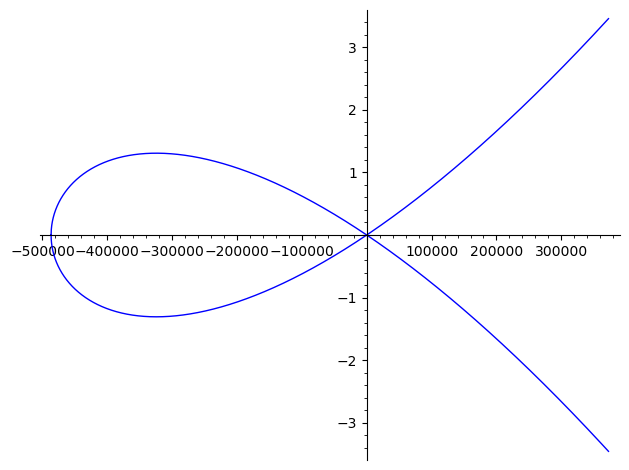
\includegraphics[width=\linewidth]{img/curve25519.png}
        \end{column}
    \end{columns}
    
\end{frame}
\begin{frame}{Gruppenstruktur}
    \begin{algorithmblock}
        \textbf{Gruppenoperationen.}\\
        Seien $P,Q\in \mathcal{E}(\mathbb{F}_{p^2})$:
         \end{algorithmblock}
        \begin{align*}
        \text{Neutrales Element}&: \; \mathcal{O}\,\text{(Punkt im Unendlichen)}\\
        \text{Punktaddition}&:P\oplus Q\\
        \text{Inverses Element}&: \ominus(x,y)=(x,-y) \\ &\quad P\oplus(\ominus P)=P\ominus P=\mathcal{O}\\
        \text{Skalarprodukt}&:[k]P=\underbrace{P\oplus\cdots\oplus P}_{k-Mal}
        \end{align*}
        
        
   
    
\end{frame}
\begin{frame}{X25519}

    \begin{definitionblock}{X25519}\\
        \vspace{-2em}
        \begin{align*}
            \mathcal{K}_{pr} &= \{0,8,16,24,\dots,248\} \times \{0,1,\dots,255\}^{30} \times \{64,65,66,\dots,127\} \\
            \mathcal{K}_{pub} &= \{0,1,\dots,255\}^{32}
        \end{align*}
        \vspace{-2em}
        \[X25519: \mathcal{K}_{pr} \times \mathcal{K}_{pub} \longrightarrow \mathcal{K}_{pub}\]
        \[(n,q)\longmapsto X([n]Q)\text{ mit $X(Q)=q$}\]
    \end{definitionblock}
    \begin{center}
        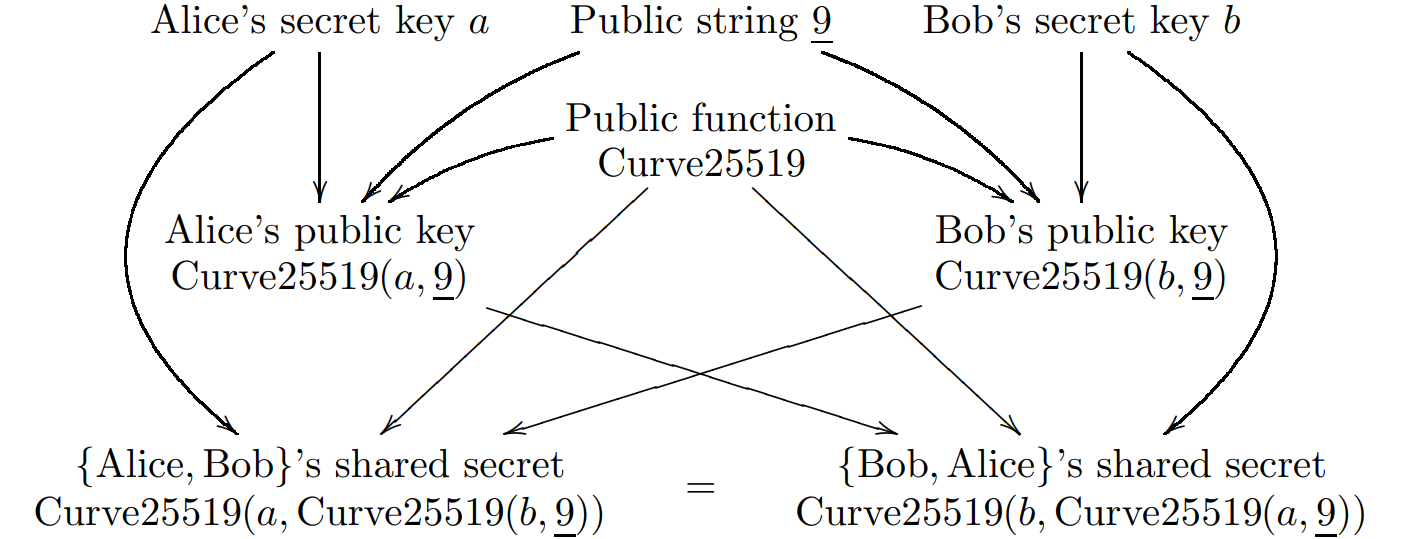
\includegraphics[width=10cm]{tex/img/d-h.png}
    \end{center}
        
\end{frame}
%\begin{frame}{Inhaltsverzeichnis}
\begin{figure}
\begin{center}
\begin{tikzpicture}
    \node (A) [nnnode, ellipse] at (4,6) {$By^2=x^3+Ax^2+x$};
    \node (B) [nnnode, ellipse] at (2,5) {$\mathbb{P}^2(\mathbb{K})$};
    \node (C) [nnnode, trapezium,trapezium left angle=70,trapezium right angle=-70,inner sep=0] at (4,4) {Montgomery Ladder};
    \node (D) [nnnode, rectangle] at (1,1){$\mathbb{F}_{2^{255}-19}{[}\sqrt{2}{]}$}
    \node (E) [nnnode, rectangle] at (1,3){$x(P)=9$}
    \node (F) [nnnode, rectangle] {$486662$}
    \node (G) [nnnode, circle split] at (5,5) {$\mathcal{K}_{pub}$ \nodepart{lower} $\mathcal{K}_{pr}$}
    \node (H) [nnnode, star, star points=13, inner sep=0, minimum width=5.5em] at (5,1) {SCA}
    \node (I) [nnnode, star, star points=13, inner sep=0, minimum width=5.5em] at (5,2) {SSCA}

    \draw[->] (A) -- (I) node [midway, yshift=7pt, bend right=60] {$\darkred{\V}$};
\end{tikzpicture}
\end{center}
\end{figure}
\end{frame}
\begin{frame}{$By^2=x^3+Ax^2+x$}
    \begin{definitionblock}{Montgomery Curve}
        \[
        \mathcal{E}_{(A,B)}:By^2=x^3+Ax^2+x, \quad B(A^2-4)\neq0
        \]
    \end{definitionblock}
    \vspace{1em}
        

    \hline
    \vspace{1em}
    \textbf{Punktoperationen}
    $P=(x_P,y_P),\;Q=(x_Q,y_Q)$
    
            
       
    \begin{columns}
    \begin{column}{0.5\linewidth}
        \begin{center}
            \textbf{Punktverdopplung}
            \begin{align*}
                x_{[2]P} &= B\lambda^2 - 2x_P - A \\
                y_{[2]P} &= \lambda(x_P - x_{[2]P}) - y_P \\
                \lambda &= (3x_P^2 + 2Ax_P + 1)/2By_P
            \end{align*}
        \end{center}
        \vfill
    \end{column}
    \begin{column}{0.5\linewidth}
        \begin{center}
            \textbf{Punktaddition}
            \begin{align*}
                x_\oplus &= B\lambda^2 - (x_P + x_Q) - A \\
                y_\oplus &= \lambda(x_P - x_\oplus) - y_P \\
                \lambda &= (y_Q - y_P)/(x_Q - x_P)
            \end{align*}
        \end{center}
        \vfill
    \end{column}
\end{columns}
    
\end{frame}
\begin{frame}{$\mathbb{P}^2(\mathbb{K})$}
    \begin{columns}
        \begin{column}{0.6\textwidth}
            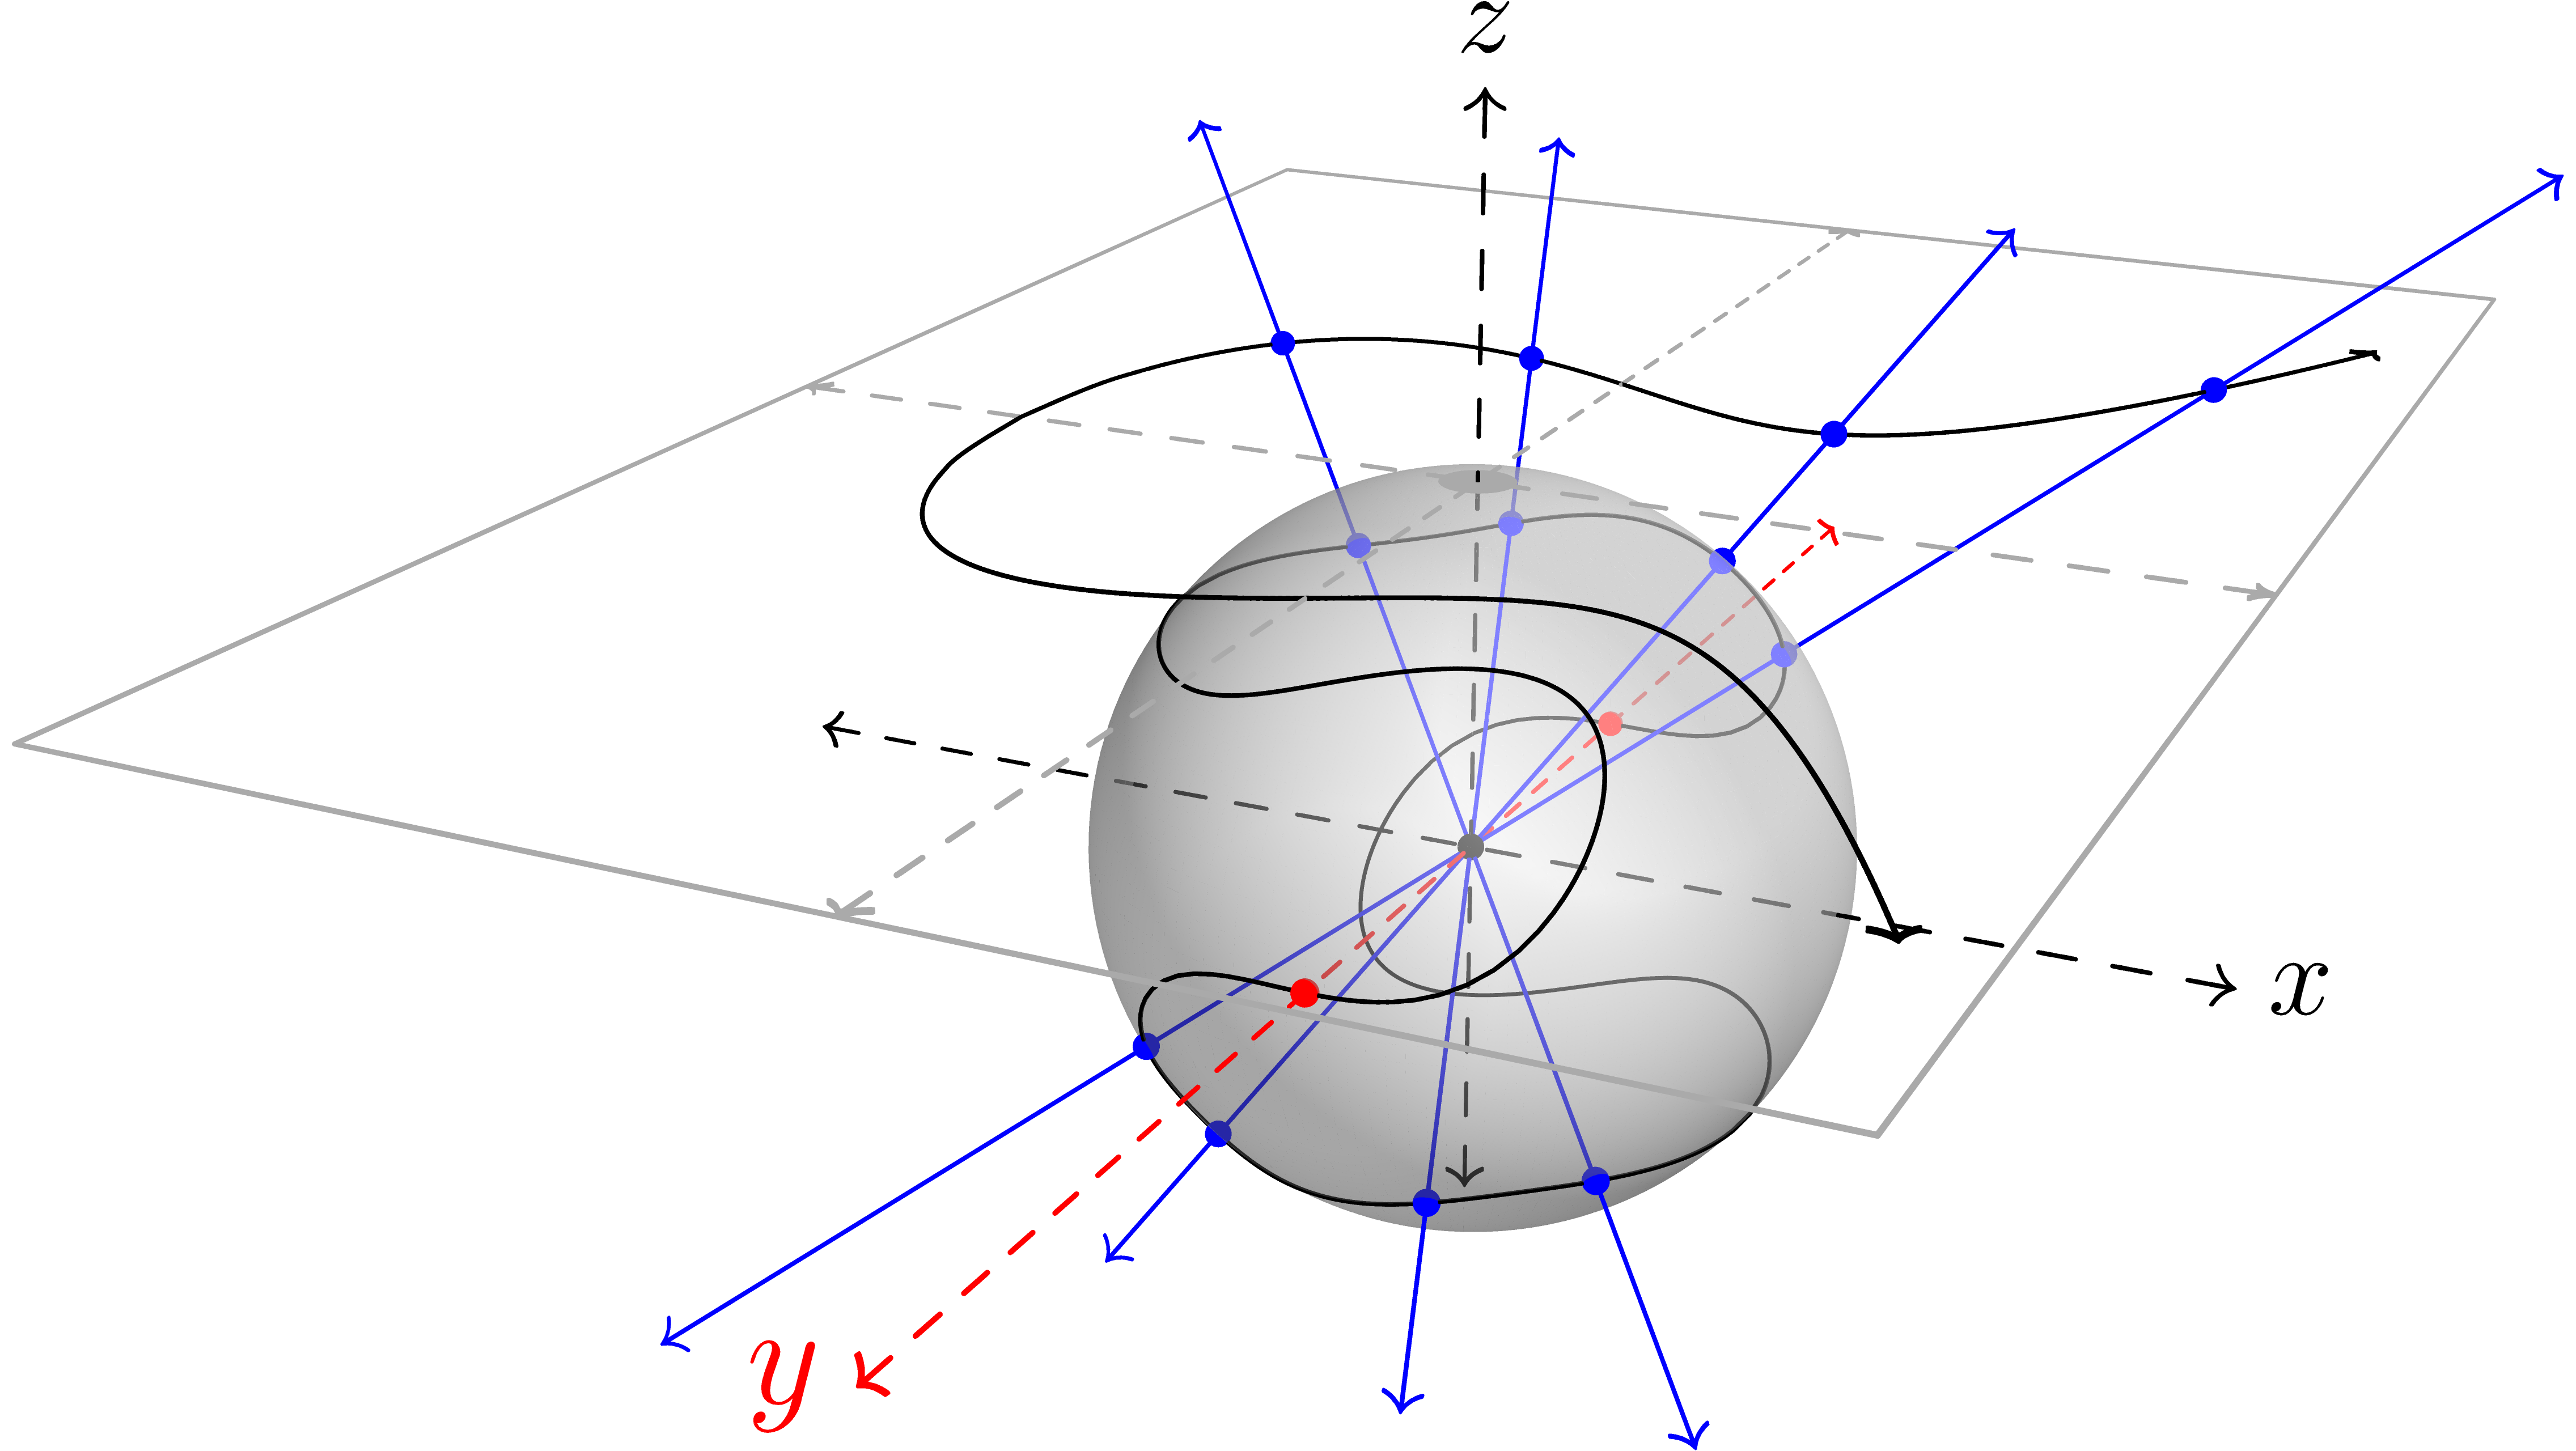
\includegraphics[width=\linewidth]{img/p^2.png}
        \end{column}
        \begin{column}{0.5\textwidth}
            \begin{definitionblock}{\\Projektiver Raum}
                \[
                    \mathbb{P}^n(\mathbb{K)} = \left( \mathbb{K}^{n+1} \setminus \{0\} \right) / \sim
                \]
                \begin{center}
                    mit der Äquivalenzrelation \\
                \end{center}
                \[
                    \sim: x \sim y \Leftrightarrow \exists \lambda \in \mathbb{K} \setminus \{0\} : x = \lambda y.
                \]
            \end{definitionblock}
            \vspace{1em}
            $P = (X:Y:Z) \in \mathbb{P}^2(\mathbb{K})$\\
            $(X:Y:Z)\sim(\lambda X:\lambda Y:\lambda Z)$
        \end{column}    
    \end{columns}
\end{frame}

\begin{frame}{$\mathbb{P}^2(\mathbb{K})$}
    \begin{columns}
        \begin{column}{0.6\textwidth}
            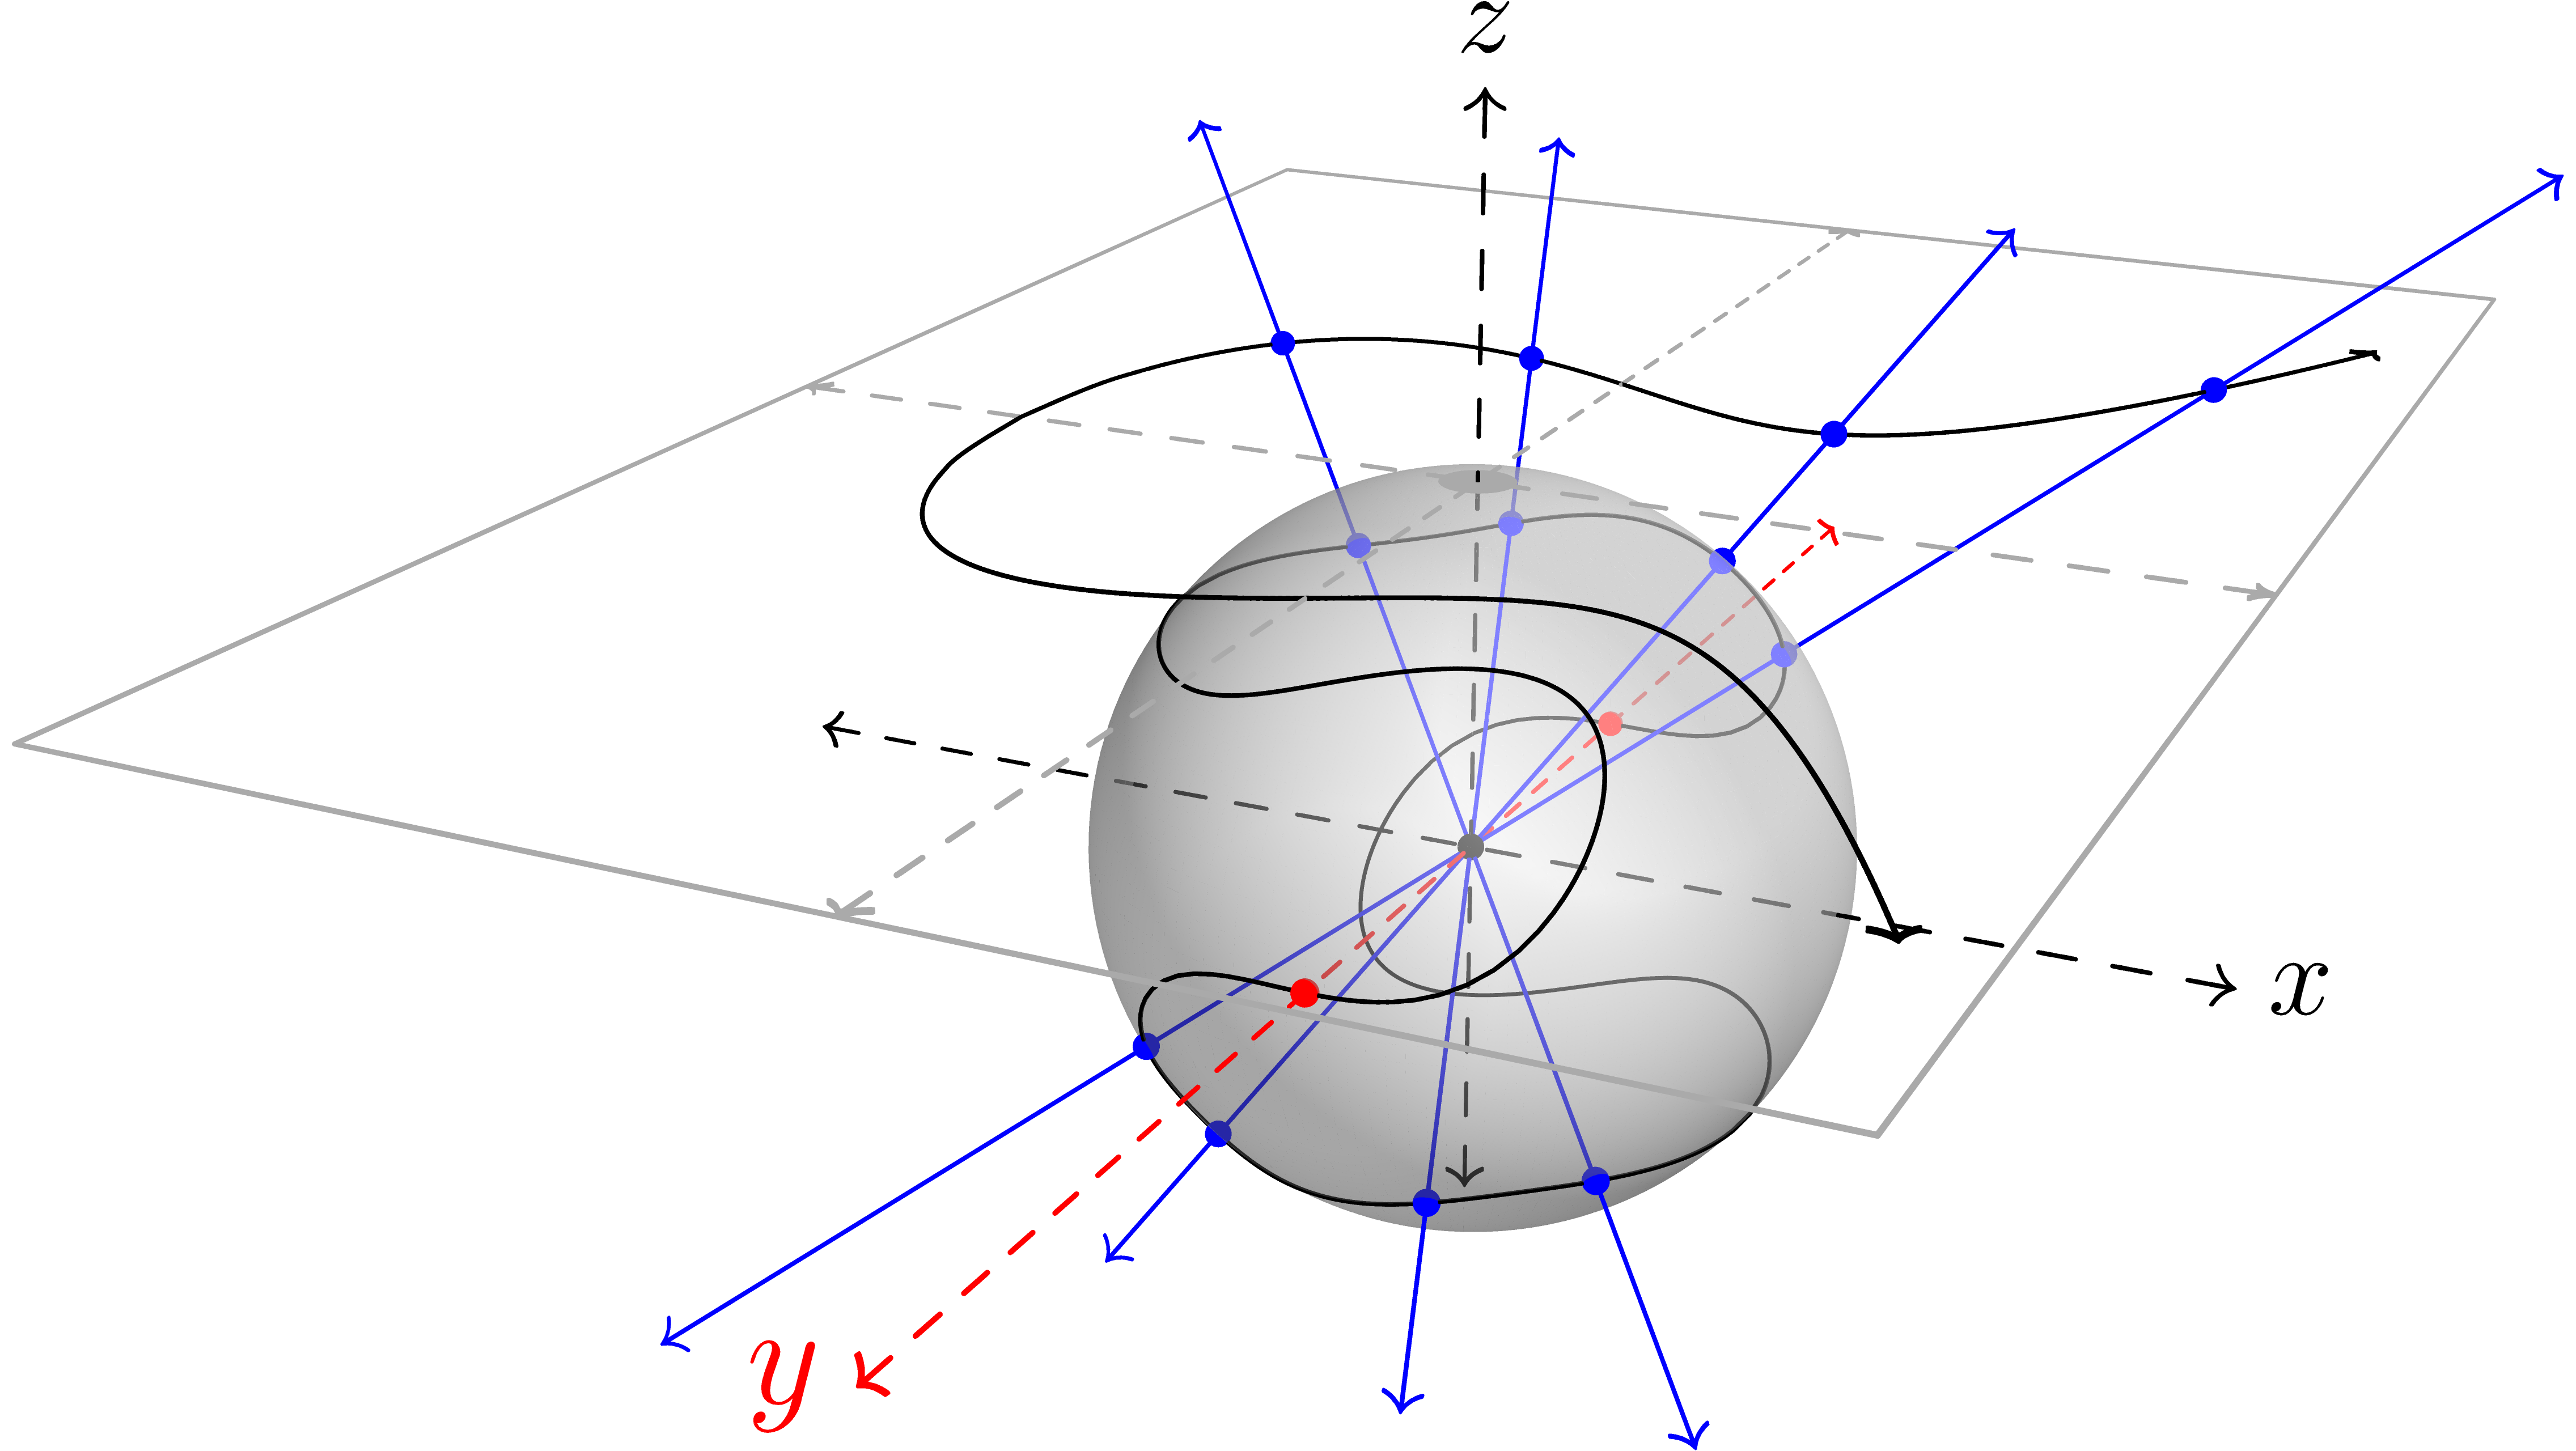
\includegraphics[width=\linewidth]{img/p^2.png}
        \end{column}
        \begin{column}{0.5\textwidth}
            \((x, y) = \left( \frac{X}{Z}, \frac{Y}{Z} \right)\)
            \[\mathcal{E}_{(A,B)}:BY^2Z=X^3+AX^2Z+XZ^2\subseteq\mathbb{P}^2\]
            \begin{algorithmblock}
                $(i)$ $Z\neq0$ \\ 
                \quad Alle Punkte der affinen Kurve liegen auf der Ebene $(x : y : 1)$\\
                $(ii)$ $Z=0\\0=X^3\Leftrightarrow X=0$ und Y beliebig\\$\mathcal{O}=(0:1:0)$
            \end{algorithmblock}
        \end{column}    
    \end{columns}
\end{frame}
\begin{frame}{Montgomery Ladder}
    \begin{definitionblock}{Montgomery Ladder}
        \\Algorithmus zur Skalarmultiplikation auf Montgomery-Kurven:
        \begin{itemize}
            \item Berechnung nur mit $x$-Koordinaten
            \item Konstante Laufzeit
        \end{itemize}
    \end{definitionblock}
    \vspace{2em}
    \[\textbf{x}:\mathcal{E}\rightarrow \mathcal{E}/\langle\ominus\rangle=\mathbb{P}^1\]
    \begin{align*}
    \textbf{x}: P \longmapsto
    \begin{cases}
        (X_P:1) & \text{für } P = (X_P:Y_P:1), \\
        (1:0) & \text{für } P = \mathcal{O} = (0:1:0).
    \end{cases}
\end{align*}
\end{frame}
\begin{frame}{Montgomery Ladder}
   
        
        
            \begin{definitionblock}{Pseudo-Operationen}
                \vspace{-1em}
                \begin{align*}
                    \texttt{xDBL:}&\textbf{x}(P)\longmapsto \textbf{x}([2]P) \\
                    \texttt{xADD:}&(\textbf{x}(P),\textbf{x}(Q),\textbf{x}(P\ominus Q))\longmapsto \textbf{x}(P\oplus Q)
                \end{align*}
                
            \end{definitionblock}
            \begin{center}
               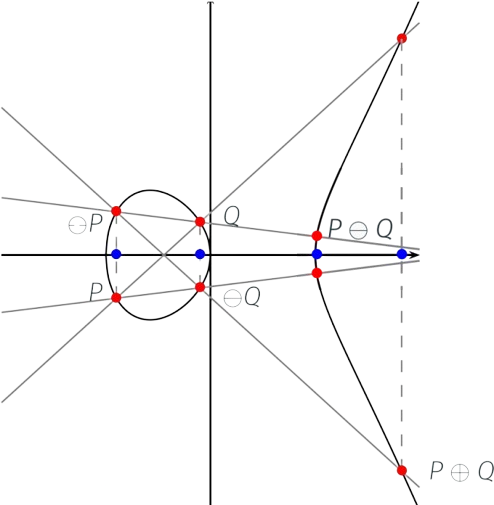
\includegraphics[width=0.35\linewidth]{img/x_cor} 
            \end{center}
       
\end{frame}
\begin{frame}{Montgomery Ladder}
    \begin{columns}
    \begin{column}{0.5\textwidth}
        \textbf{\texttt{xDBL}}\\
    \vspace{-1.8em}
    \begin{align*}
        x_{[2]P}&=B\lambda^2-2x_P-A\\
        &=\frac{(3x_P+2Ax_P+1)^2}{4By^2_P}\\&\quad-2x_P-A\\
        &=\frac{(x_P^2-1)^2}{4(x_P^3+Ax_P^2+x_P)}
    \end{align*}
    \end{column}
    \begin{column}{0.5\linewidth}
    \begin{align*}
        \textbf{\texttt{xADD}}\\
        &x_{P\oplus Q} x_{P\ominus Q}\\
        &= \left(B\left(\frac{(y_Q - y_P)^2}{(x_Q - x_P)^2}\right)  - (x_P + x_Q)-A\right)\\
        &\quad\cdot\left(B\left(\frac{(-y_Q - y_P)^2}{(x_Q - x_P)^2}\right)  - (x_P + x_Q)-A\right)\\
        &=  \frac{(x_Qx_P-1)^2}{(x_Q-x_P)^2}
    \end{align*}
    \end{column}
        
    \end{columns}
    \begin{itemize}
        \item Inversionen sind in endlichen Körpern rechenintensiv
        \item Projektive Koordinaten vermeiden direkte Inversion
        \item Darstellung der $x$-Koordinate als Bruch $\frac{X}{Z}$
        \item Rückwandlung in die affine Koordinate durch $x=XZ^{p-2}$
    \end{itemize}
    
\end{frame}

\begin{frame}{Montgomery Ladder}
    \begin{algorithmblock}
    \textbf{Notation}\\
    \vspace{-1.5em}
    \begin{center}
        $(X_P:Z_P)\coloneqq\textbf{x}(P),$ \quad $(X_Q:Z_Q)\coloneqq\textbf{x}(Q)$ \\
        \vspace{1em}
        $(X_\oplus:Z_\oplus)\coloneqq\textbf{x}(P\oplus Q),$ \quad $(X_\ominus:Z_\ominus)\coloneqq\textbf{x}(P\ominus Q)$
    \end{center}
    \end{algorithmblock}
    \vspace{1em}
    \begin{columns}
        \begin{column}{0.5\textwidth}
            \textbf{\texttt{xDBL}}
            \begin{align*}
                X_{[2]P} &= (X_P^2-Z_P^2)^2 \\
                Z_{[2]P} &= 4X_PZ_P(X_P^2+AX_PZ_P+Z_P^2)
\end{align*}
            
        \end{column}
        \begin{column}{0.5\textwidth}
            \textbf{\texttt{xADD}}
            \begin{align*}
                X_{\oplus} &= 4(X_PX_Q-Z_PZ_Q)Z_{\ominus} \\
                Z_{\oplus} &= 4(X_PZ_Q - Z_PX_Q)X_\ominus
            \end{align*}
        \end{column}
    \end{columns}
\end{frame}

\begin{frame}{Montgomery Ladder}
    \begin{columns}
        \begin{column}{0.4\textwidth}
            \textbf{\texttt{xDBL}}
            \begin{align*}
                X_{[2]P} &= (X_P + Z_P)^2 (X_P - Z_P)^2 \\
                Z_{[2]P} &= (4X_PZ_P)((X_P - Z_P)^2 \\ &\quad+ \left((A + 2)/4)(4X_PZ_P)\right)
\end{align*} \\
\textbf{\texttt{xADD}}
            \begin{align*}
                X_{\oplus} &= Z_{\ominus} [ (X_P - Z_P)(X_Q + Z_Q) \\
                & \quad + (X_P + Z_P)(X_Q - Z_Q) ]^2 \\
                Z_{\oplus} &= X_{\ominus} [ (X_P - Z_P)(X_Q + Z_Q) \\
                &\quad - (X_P + Z_P)(X_Q - Z_Q) ]^2
                \end{align*}
            
        \end{column}
        \begin{column}{0.7\textwidth}
            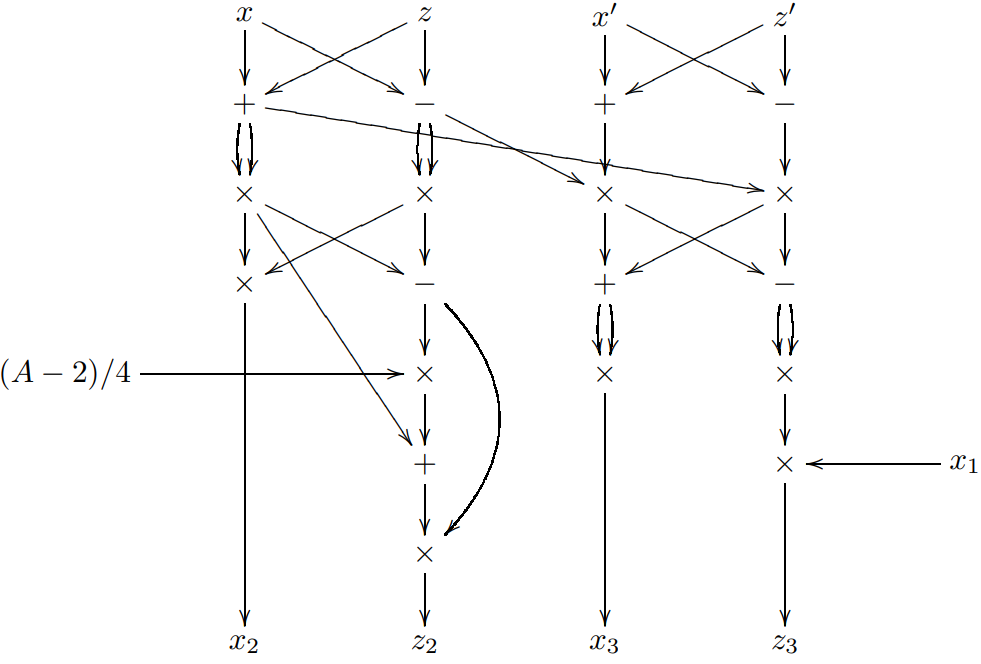
\includegraphics[width=1\textwidth]{tex/img/ladder.png}
      
        \end{column}
    \end{columns}
    
\end{frame}

\begin{frame}{Montgomery Ladder}
    \begin{algorithm}[H]
        \caption{\textbf{Algorithmus: Montgomery Ladder}}
        
        
        \textbf{Input:} $(1)\ k=\sum\nolimits_{i=0}^{l-1}k_i2^i$ mit $k_{l-1}=1$ \hfill \texttt{//Binärdarstellung des Skalars} \\ 
        \text{} $\quad \quad \quad \; (2)\ (X_P,Z_P)$, so dass $(X_P:Z_P)=\textbf{x}(P)$ \\
        \textbf{Output:} $(X_k,Z_k)$, so dass $(X_k:Z_k)=\textbf{x}([k]P)$
        
        \begin{algorithmic}[1]
            \State $\texttt{(x$_0$,x$_1$)} \gets ((X_P, Z_P), \texttt{xDBL}(X_P, Z_P))$ \hfill \texttt{//x$_1$-x$_0$ ist immer $(X_P,Z_P)$} \\
            \textbf{for} $i = l-2$ \textbf{downto} 0 \textbf{do}\\
            \quad \textbf{if} $k_i = 0$ \textbf{then}
            \State \quad \quad $\texttt{(x$_0$,x$_1$)} \gets (\texttt{xDBL}(\texttt{x$_0$}),\texttt{xADD}(\texttt{x$_0$},\texttt{x$_1$},(X_P,Z_P)))$ \\
            \quad \textbf{else}
            \State \quad \quad $\texttt{(x$_0$,x$_1$)} \gets (\texttt{xADD}(\texttt{x$_0$},\texttt{x$_1$},(X_P,Z_P)),\texttt{xDBL}(\texttt{x$_1$}))$
            \State \textbf{return} $\texttt{x$_0$}$ \hfill \texttt{//x$_0$}$=\textbf{x}([k]P)$, \texttt{x$_0$}$=\textbf{x}([k+1]P)$
            
         
        \end{algorithmic}
    \end{algorithm}
    
\end{frame}


\begin{frame}{SCA}
    \begin{definitionblock}{Side-channel attack}
        \\ Angriff, der physische Informationen wie Zeit oder Stromverbrauch nutzt, um geheime Daten aus einem kryptographischen System zu erhalten
    \end{definitionblock}
    \vspace{1em}
    Beispiele Schwachstellen:
    \begin{itemize}
        \item Verzweigungen basierend auf geheimen Bits\\
        z.B. if($\texttt{b$_i$}==0$): mit \texttt{b} geheim
        \item Speicherzugriff mit einem geheimen Index
        z.B. $\texttt{x}=\texttt{T}[\texttt{b}]$ mit \texttt{b} geheim
    \end{itemize}
\end{frame}
\begin{frame}{Montgomery Ladder}
    \begin{algorithm}[H]
        \caption{\textbf{\texttt{SWAP()}} – Bedingter Tausch in konstanter Zeit}
        
        \textbf{Input:} $(1) \ b \in \{0,1\}$\\
        \text{} $\quad \quad \quad \; (2) \ \texttt{(x$_0$,x$_1$)}$ \hfill \texttt{//x$_0$ und x$_1$ als n-bit Strings} \\
        \textbf{Output:} $\texttt{(x$_b$,x$_{b-1}$)}$
        
        \begin{algorithmic}[1]  
            \State \hspace{0.5cm} $\texttt{b} \gets (b,\dots,b)_n$
            \State \hspace{0.5cm} $\texttt{v} \gets \texttt{b}\land\texttt{(x$_0$ xor x$_1$)}$
            \State \textbf{return} $\texttt{(x$_0$ xor v, x$_1$ xor v)}$
        \end{algorithmic}
    \end{algorithm}    
\end{frame}

\begin{frame}{Montgomery Ladder}
    \begin{algorithm}[H]
        \caption{\textbf{Algorithmus: Montgomery Ladder mit \texttt{SWAP()}}}
        
        
        \textbf{Input:} $(1)\ k=\sum\nolimits_{i=0}^{l-1}k_i2^i$ mit $k_{l-1}=1$  \\ 
        \text{} $\quad \quad \quad \; (2)\ (X_P,Z_P)$, so dass $(X_P:Z_P)=\textbf{x}(P)$ \\
        \textbf{Output:} $(X_k,Z_k)$, so dass $(X_k:Z_k)=\textbf{x}([k]P)$
        
        \begin{algorithmic}[1]
            \State $\texttt{(x$_0$,x$_1$)} \gets ((X_P, Z_P), \texttt{xDBL}(X_P, Z_P))$ \\
            \textbf{for} $i = l-2$ \textbf{downto} 0 \textbf{do}
            \State \quad $\texttt{(x$_0$,x$_1$)} \gets \texttt{SWAP}((k_{i+1} \texttt{ xor } k_i),\texttt{(x$_0$,x$_1$)})$
            \State \quad $\texttt{(x$_0$,x$_1$)} \gets (\texttt{xDBL}(\texttt{x$_0$}),\texttt{xADD}(\texttt{x$_0$},\texttt{x$_1$},(X_P,Z_P)))$
            \State $\texttt{(x$_0$,x$_1$)} \gets \texttt{SWAP}(k_0,\texttt{(x$_0$,x$_1$)})$
            \State \textbf{return} $\texttt{x$_0$}$ 
            
         
        \end{algorithmic}
    \end{algorithm}
    
\end{frame}

\begin{frame}{$\mathbb{F}_{p^2}$}
    \begin{definitionblock}{$\mathbb{F}_{p^2}$}
        \\ Sei $\delta$ das kleinste nicht-quadratische Element in $\mathbb{F}_p$.\\
        Dann ist die quadratische Erweiterung von $\mathbb{F}_p$ definiert als
        \[\mathbb{F}_{p^2} =\mathbb{F}_p(\sqrt{\delta})=\{a+b\sqrt{\delta} \mid a,b\in \mathbb{F}_p\}.\]
    \end{definitionblock}
    \vspace{1em}
    \textbf{Bemerkung:}\\
    \begin{itemize}
        \item Ganau $(p-1)/2$ nicht-quadratische Zahlen in $\mathbb{F}_p$
        \item $\alpha$ ist nicht-quadratisch $\Leftrightarrow$  $\alpha/\delta$ ist eine Quadratzahl 
    \end{itemize}
    
\end{frame}

\begin{frame}{$\mathbb{F}_{p^2}$}
    \textbf{Reguläre Kurve:}\\
    $\mathcal{E}_A:y^2=x^3+Ax^2+x$\quad über $\mathbb{F}_p$\\
    $\mathcal{E}^\prime(\mathbb{F}_{p^2})=\{\mathcal{O}\}\cup (\mathcal{E}(\mathbb{F}_{p^2})\cap (\mathbb{F}_p\times\mathbb{F}_p))$
    $\mathcal{E}_A:y^2=x^3+Ax^2+x$\\
    \vspace{1em}
    \textbf{Quadratischer Twist:}\\
    $\mathcal{E}_{(A,B)}:By^2=x^3+Ax^2+x$\quad über $\mathbb{F}_p$ (B nicht-quadratisch)\\
    $\mathcal{E}^{\prime\prime}(\mathbb{F}_{p^2})=\{\mathcal{O}\}\cup (\mathcal{E}(\mathbb{F}_{p^2})\cap (\mathbb{F}_p\times\sqrt{\delta}\mathbb{F}_p))$
    \[\mathcal{E}(\mathbb{F}_{p^2})=\mathcal{E}^\prime(\mathbb{F}_{p^2})\cup\mathcal{E}^{\prime\prime}(\mathbb{F}_{p^2})\]
    \begin{center}
        Montgomery Ladder auf der regulären Kurve und \\ihrem quadratischen Twist gleich, da sie nicht von B abhängig ist
    \end{center}
\end{frame}
\begin{frame}{$\mathcal{K}_{pub}$}
    \[\mathcal{K}_{pub} = \{0,1,\dots,255\}^{32}\] \\
    \begin{center}
        keine Validierung des öffentlichen Schlüssels notwendig
    \end{center}
\end{frame} 
\begin{frame}{$2^{255}-19$}
\textbf{Bedingungen:}
    \begin{itemize}
        \item Primzahl nahe einer Zweierpotenz
        \begin{itemize}
            \item Schnelle Modulo-Berechnungen
        \end{itemize}
        \item Knapp unter 32k Bits (k: Ganzzahl)
            \begin{itemize}
                \item Öffentlicher Schlüssel kann als 32-bit Words mit geringer Speicherverschwendung übermittelt werden
            \end{itemize}
    \end{itemize}
\textbf{Optionen:}
\[\{2^{255}+95,2^{255}-19,2^{255}-31, 2^{254}+79,2^{253}+51, 2^{253}+39\}\]
\[\textbf{2$^{\textbf{255}}$-19}\text{, da 19 kleiner als 31,39,51,79,95}\]
\end{frame}
\begin{frame}{$X(P)=9$}
    \begin{algorithmblock}{\textbf{Satz: Satz von Lagrange.}}
        Sei $G$ eine endliche Gruppe und $H$ eine Untergruppe von $G$. Dann gilt
        \[\#H \mid \#G.\]
    \end{algorithmblock}
    \vspace{1em}
    Für jeden Punkt $Q\in \mathcal{E}^\prime(\mathbb{F}_{p^2})$ gilt folglich:
    \[ \#\langle Q\rangle \in \{1,2,4,8,l,2l,4l,8l\}\] 
     \[(\#\mathcal{E}^\prime(F_{p^2})=8l)\]
     \vspace{-1em}
     \begin{itemize}
         \item $1,2,4,8$ zu klein
         \item Vielfache von $l$ für den Pohlig-Hellman-Algorithmus anfällig\\
         \rightarrow nur $l$ geeignet
     \end{itemize}
     
     
     
    
    \begin{center}
    \fbox{%
        \parbox{0.65\textwidth}{%
            \vspace{-1.5em}
            \begin{align*}
            X(P) &= \min\{x \mid Q = (x,y) \in \mathcal{E}^\prime(\mathbb{F}_{p^2}),\ \#\langle Q \rangle = l\} \\
            &= 9
            \end{align*}
            \vspace{-2em}
        }%
    }
    \end{center}


\end{frame}
\begin{frame}{SSCA}
    \begin{definitionblock}{Small subgroup confinement attack}
        \\Angriff, der kleine Untergruppen nutzt, um Teile des privaten Schlüssels zu enthüllen
        
     \end{definitionblock}
     \vspace{1em}
     \textit{Beispiele}:
        \begin{itemize}
            \item Pohlig-Hellman-Algorithmus: Nur wenn $\#\langle P \rangle$ eine zusammengesetzte Zahl ist
            \item Ungültiger Generator: Bewusste Auswahl eines Generator aus einer kleinen Untergruppe
                           
        \end{itemize}
            \begin{align*}
                 \text{Öffentlicher Schlüssel von B}&:H\text{, Generator einer kleinen Untergruppe}\\
                \text{Gemeinsamer Schlüssel von A}&:aH\text{, welcher ebenfalls in der Untergruppe liegt}
            \end{align*}
            \[a\mod{\#\langle H\rangle}\]

   
\end{frame}

\begin{frame}{$\mathcal{K}_{pr}$}
    \begin{algorithm}[H]
        \caption{\textbf{\texttt{CLAMP()}} – Anpassung des Skalars für X25519}
        \label{alg:clamp}
        
        \textbf{Input:} $k \in \{0,1,\dots,255\}^{32}$ \hfill \texttt{// 32-Byte zufällig generierter Wert}\\
        \textbf{Output:} Angepasster Skalar $k'$
        
        \begin{algorithmic}[1]  
            \State \hspace{0.5cm} $\texttt{k{[}0{]}} \gets \texttt{k{[}0{]}} \land 248$ \hfill \texttt{// 248 = (11111000)$_\texttt{2}$}
            \State \hspace{0.5cm} $\texttt{k{[}31{]}} \gets \texttt{k{[}31{]}} \land 127$ \hfill \texttt{// 127 = (01111111)$_\texttt{2}$}
            \State \hspace{0.5cm} $\texttt{k{[}31{]}} \gets \texttt{k{[}31{]}} \lor 64$ \hfill \texttt{// \ 64 = (01000000)$_\texttt{2}$}
            \State \hspace{0.5cm} $\texttt{k'} \gets \texttt{k}$
            \State \hspace{0.5cm} $\textbf{return} \ \texttt{k'}$
        \end{algorithmic}
    \end{algorithm}
\end{frame}

\begin{frame}{$\mathcal{K}_{pr}$}
    \begin{tabular}{c|c|c}
       \texttt{1:} \;$\; \texttt{k[0]} \land \texttt{(11111000)$_2$ }$  & Niedrigstwertige 3 Bits $\gets 0$ & $8\mid \texttt{k}$\\
       \texttt{2:} $\texttt{k[31]} \land \texttt{(01111111)$_2$ }$  & Das höchstwertige Bit $\gets 0$&$\texttt{k}\leq2^{255}-1$\\
       \texttt{3:} $\texttt{k[31]} \lor \texttt{(01000000)$_2$ }$ & Das zweithöchstwertige Bit $\gets 1$&$\texttt{k}\geq2^{254}$
       
    \end{tabular}
    \begin{align*}
        \mathcal{K}_{pr}&= \{0,8,16,24,\cdots,248\} \times \{0,1,\cdots,255\}^{30} \times \{64,65,66,\cdots,127\} \\
        &={\{\underline{n}:n\in 2^{254}+8\{0,1,\dots,2^{251}-1\}\}}
    \end{align*}
    \vspace{-1.5em}
    \begin{algorithmblock}
        \begin{itemize}
            \item SSCA: $\texttt{k}\equiv0\mod{2^i}$ für $1\leq i\leq 3$
            \item Vermeidung von kleinen Skalaren\\
            \item Skalar zwischen $2^{251}$ und $2^{252}-1$($\approx\#\langle P\rangle$)\\(Verschiebung von 3 Bits durch Faktor 8) \rightarrow $2^{254}\leq \texttt{k} \leq 2^{255}-1$
            \item SCA: Feste effektive Schlüssellänge von 255 Bits erzwingt konstante Iterationen 
        \end{itemize}
    \end{algorithmblock}
    
\end{frame}



\begin{frame}{486662}
\textbf{Bedingungen:}
    \begin{itemize}
        \item $(A-2)/4$ kleine Ganzzahl (Montgomery Ladder)
        \item $\#\mathcal{E}^\prime(\mathbb{F}_{p^2})=8l_1$ 
        \item $\#\mathcal{E}^{\prime\prime}(\mathbb{F}_{p^2})=4l_2$
    \end{itemize}
\textbf{Optionen:}
    \[\{358990,464586,486662\}\]
    \[\textbf{486662}\text{, da sonst $l_1$ oder $l_2$ kleiner als $2^{252}$}\]
\end{frame}

\begin{frame}{Quellen}
    \begin{enumerate}[ {[}1{]} ]
        \item Daniel J. Bernstein, Curve25519: new Diffie-Hellman speed records, 2006. 
        \item Craig Costello and Benjamin Smith, Montgomery curves and their arithmetic: The case of large characteristic fields, 2017.
        \item Daniel J. Bernstein and Tanja Lange, Montgomery curves and the Montgomery ladder, 2017.
        \item Risen Crypto, Clamping \& Cofactor clearing in Curve25519, 2022, https://risencrypto.github.io/CofactorClearing - (28.03.2025 23:10).
        \item SafeCurve, choosing safe curves for elliptic-curve cryptography, 2013, https://safecurves.cr.yp.to/twist.html - (29.03.2025 21:02). 
    \end{enumerate}
\end{frame}


\end{document}